\documentclass[12pt,a4paper]{article}

\usepackage[english]{babel}
\usepackage[utf8]{inputenc}     % Für Umlaute
\usepackage[T1]{fontenc}        % Saubere Schriftkodierung
\usepackage{lmodern}            % Bessere Schriftarten
\usepackage{helvet}
\renewcommand{\familydefault}{\sfdefault}
\usepackage{graphicx}           % Für Bilder
\usepackage{plantuml}
\usepackage{hyperref}           % Für klickbare Links
\usepackage[letterpaper, top=2cm, bottom=2cm, left=2cm, right=2cm, marginparwidth=1.75cm]{geometry}
\usepackage{amsmath}
\usepackage{graphicx}
\usepackage{enumitem}

\title{Test Interface für HAL Tests auf dem Target}
\author{Konrad Wöhrle}
\date{\today}

%==================================================================
\begin{document}

\maketitle
\tableofcontents
\newpage
%==================================================================
%________________________________
\section{Einleitung}
%______________________
\subsection{Anforderungen}
%____________
\subsubsection{Motivation und Zielsetzung}


%____________
\subsubsection{Aufgabenblatt}
\textbf{Google-Test Interface für HAL-Tests auf dem Target}
\newline
Google-Test ist ein etabliertes Tool für Unit-Tests und hat sich in vielen Bereichen der C++-Software-Entwicklung verbreitet. Im Embedded Bereich können damit die oberen Abstraktionsschichten einer Software getestet werden. Google-Test ist ein großes Framework und deshalb nicht (oder nur bedingt) geeignet auf den begrenzten Ressourcen eines Micro-Controllers zu laufen. Unit-Tests der HAL (Hardware Abstraction Layer) sind deshalb selten möglich.
Die Fa. MicroConsult, bekannt durch Trainings für die Software-Entwicklung, bietet eine Lösung an. Diese nennt sich 'wogtest' (Without Googletest). Es bietet eine leichtgewichtige Lösung, die Google-Test-Befehle versteht. Dabei wird nur ein include benötigt. Die zugehörige Implementierung muss für die jeweilige Zielplattform erstellt werden.
Wogtest ist frei und kostenlos samt Doku im Download von Microconsult erhältlich.
\newline\newline
\textbf{Die Herausforderung}
\newline
Verschiedene Aspekte der Software-Entwicklung werden berührt und vertieft. Dazu gehören neben dem eigentlichen Test-Projekt auch Bereiche, die den Projektaufbau und die Build-Umgebung, sowie die Toolchain betreffen. 
\newline

\textbf{Aufgaben}
\begin{enumerate}
  \item Vorhandenes Google-Test-Template in Betrieb nehmen unter Linux (wsl)
  \item Anlegen eines (lokalen) Git-Repositories
  \item Inbetriebnahme eines Micro-Controller-Boards (z.B. STM-Nucleo) mit einer kleinen Beispielapplikation (Blinky). Debugging, Flashen, …
  \item Implementierung der Funktionen aus dem 'wogtest'-include-File
  \item Aufbau eines Test-Templates für eine HAL-Komponente mit vorgegebenem Micro-Controller
  \item Stubbing und Mocking in Tests
  \item Erstellen einer Ausgabe-Schnittstelle für die Testergebnisse, z.B. über Segger RTT
  \item Erzeugen eines Test-Reports
  \item Erstellung der Dokumentation inklusive Anleitung im Markup-Format
  \item Optional: Umbau der Build-Umgebung zu einem Docker-Container\newline
\end{enumerate}
\textbf{Voraussetzung}
\newline
Grundkenntnisse in und Spaß an der hardwarenahen Software-Entwicklung.

%____________
\subsubsection{}
%______________________
\subsection{Übersicht Aufgabenstellung}

\empty

\newpage
%==================================================================
%________________________________
\section{Planung}
%______________________
\subsection{Tatsächlicher Projektablauf}
\begin{itemize}
  \item Vorhandene Testumgebung in Betrieb nehmen
  \item Microcontroller in Betrieb nehmen (PlatformIO)
  \item Git-Repositories anlegen
  \item einlesen in CMake
  \item LED Blink Programm (später Taster einbinden) / Architektur mit Application, Treiber und Hardwareschicht
  \item Google Test auf Host (inclusive Stubbing)
  \item Hterm in Betrieb nehmen (Von Hterm an Controller senden und wieder zurück)
  \item per printf an Hterm senden (printf umleiten)
  \item Test für Target schreiben (wogtest)

\end{itemize}

\begin{figure}[htbp]
  \centering
  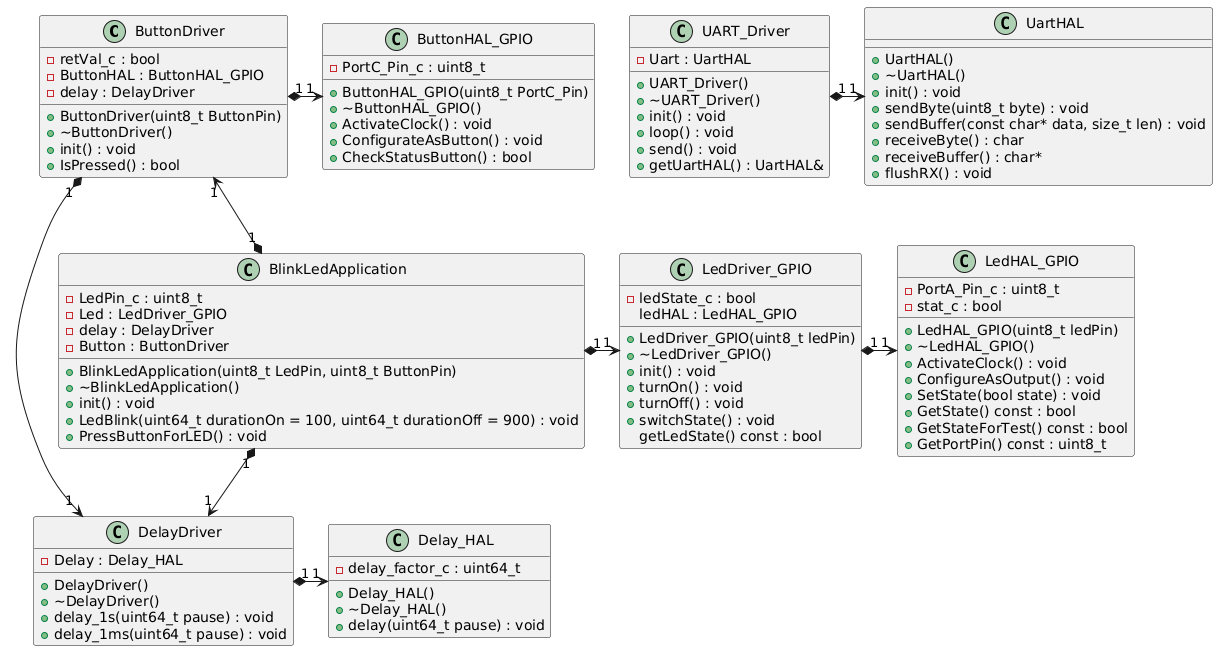
\includegraphics[width=\textwidth]{LED_Blink_UML.png}
  \caption{UMLKlassendiagramm}
  \label{fig:uml_led_blink}
\end{figure}

\newpage
%==================================================================
%________________________________
\section{Bedienungsanleitung}
%______________________
\subsection{Beispielapplikation}
\begin{verbatim}

    if(ButtonPressed)
    {
        ledState = ! ledState;
    }

\end{verbatim}

Your Abstractö qwfq wbo9qbvf9 quzwvauvbza ibzuvbEFH UZBoac BZBuzbviu eb vububIUBVDubbvvd Bb bdcub I UBCu bUB UBVI bvuz ubdvsdzbvVUZBVDB BU B b  biSDBVZUIB VuzsbdviszudaizsudhI D IUZBi


\textbf{Das ist fett.}
\textit{Das ist kursiv.}
\textbf{\textit{Fett und kursiv!}}


\end{document}